% Lokale Stile für dieses Kapitel (ändern keine globalen Einstellungen)
\pgfplotsset{
    linfkt/.style={
            axis lines=middle,
            axis line style={->},
            xlabel={$x$}, ylabel={$y$},
            xtick distance=1, ytick distance=1,
            grid=both,
            grid style={lightgray!40},
            tick label style={font=\scriptsize},
            label style={font=\small},
            enlargelimits=false,
        },
    linfktpunkt/.style={
            axis lines=middle,
            axis line style={->},
            xlabel={$x$}, ylabel={$y$},
            xtick distance=1, ytick distance=1,
            grid=both,
            major grid style={line width=0.6pt, draw=black!60, dotted},
            tick label style={font=\scriptsize},
            label style={font=\small},
            enlargelimits=false,
        },
}

\section{Lineare Funktionen}
\subsection{Einstiegsaufgaben}
\subsubsection*{Einstiegsaufgabe 1}
\begin{minipage}{0.8\textwidth}
    Um zum Flughafen zu gelangen, planen Alice und Bob, ein Taxi zu mieten. Dazu erkundigen sie sich bei zwei verschiedenen Taxiunternehmen nach den Tarifen.

    \smallskip
    Bei \textit{Max-Taxi} gibt es eine Grundgebühr von 5 CHF und für jeden gefahrenen Kilometer bezahlt man zusätzlich 3.50 CHF.

    \smallskip
    Bei \textit{Prestige-Taxi} beträgt die Grundgebühr 10 CHF. Pro gefahrenen Kilometer werden dafür nur 3 CHF verlangt.
\end{minipage}\hfill
\begin{minipage}{0.17\textwidth}
    
\includegraphics[width=\textwidth]{LineareFunktionen/im/Taxi.png}
\end{minipage}

\begin{enumerate}
    \item Geben Sie die Gleichung der beiden Funktionen $M(s)$ und $P(s)$ an, welche der zurückgelegten Strecke $s$ (in Kilometer) den Fahrpreis für die beiden Unternehmen Max-Taxi und Prestige-Taxi zuordnen.\\[0.4cm]
          $M(s) =$\\[0.8cm]
          $P(s) =$\\[0.4cm]
    \item Betrachten Sie nun die Graphen der beiden Funktionen $M(s)$ und $P(s)$.
          \begin{center}
              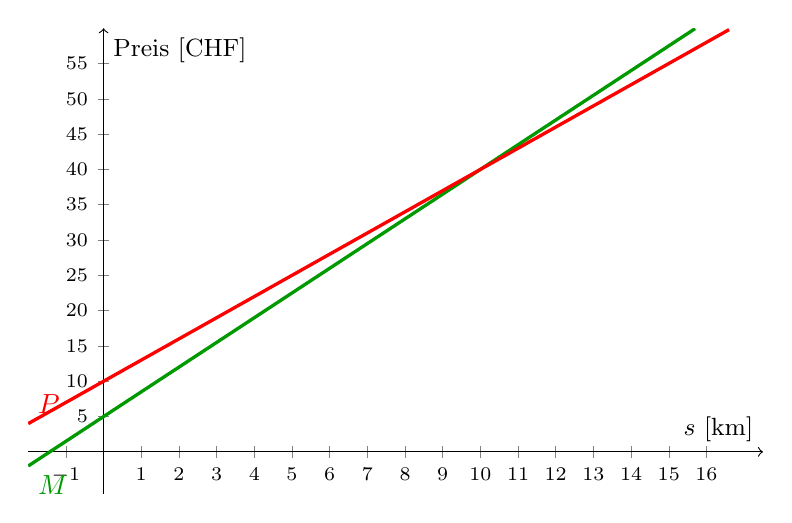
\begin{tikzpicture}
                  \begin{axis}[
                          axis lines=middle,
                          axis line style={->},
                          width=0.9\linewidth, height=7.5cm,
                          xlabel={$s$ [km]}, ylabel={Preis [CHF]},
                          xmin=-2, xmax=17.5,
                          ymin=-6, ymax=60,
                          xtick={-1,1,2,...,16},
                          ytick={5,10,...,55},
                          tick label style={font=\scriptsize},
                          label style={font=\small},
                          enlargelimits=false,
                      ]
                      \addplot[domain=-2:15.7, very thick, green!60!black] {3.5*x+5};
                      \addplot[domain=-2:16.6, very thick, red] {3*x+10};
                      \node[green!60!black, below right] at (axis cs:-2,-2) {$M$};
                      \node[red, above right] at (axis cs:-2,4) {$P$};
                  \end{axis}
              \end{tikzpicture}
          \end{center}
          \begin{enumerate}
              \item Wie können am Graphen die Grundgebühren der beiden Taxi-Unternehmen abgelesen werden?
              \item Wie können am Graphen die Kosten pro Kilometer der beiden Taxi-Unternehmen abgelesen werden?
          \end{enumerate}
    \item Wie kann man herausfinden, ab wie vielen Kilometern das eine Unternehmen günstiger als das andere ist? Kann man das nur graphisch herausfinden oder auch rechnerisch? Welcher Weg hat welche Vorteile?
    \item Bei den beiden Graphen handelt es sich um Geraden. Was könnte der Grund dafür sein?
\end{enumerate}
\newpage
\subsubsection*{Einstiegsaufgabe 2}
\begin{mdframed}[linewidth=1pt, innerleftmargin=10pt, innerrightmargin=10pt, innertopmargin=10pt, innerbottommargin=10pt]
    \textbf{\underline{Wie steil ist die Gerade?}}

    \medskip
    Alice hat die folgende Abbildung einiger Geraden vor sich. Sie ruft gleich Bob an, der die Graphik nicht sieht, und möchte ihm erzählen, wie die Geraden aussehen und insbesondere, wie steil sie sind.
    \begin{center}
        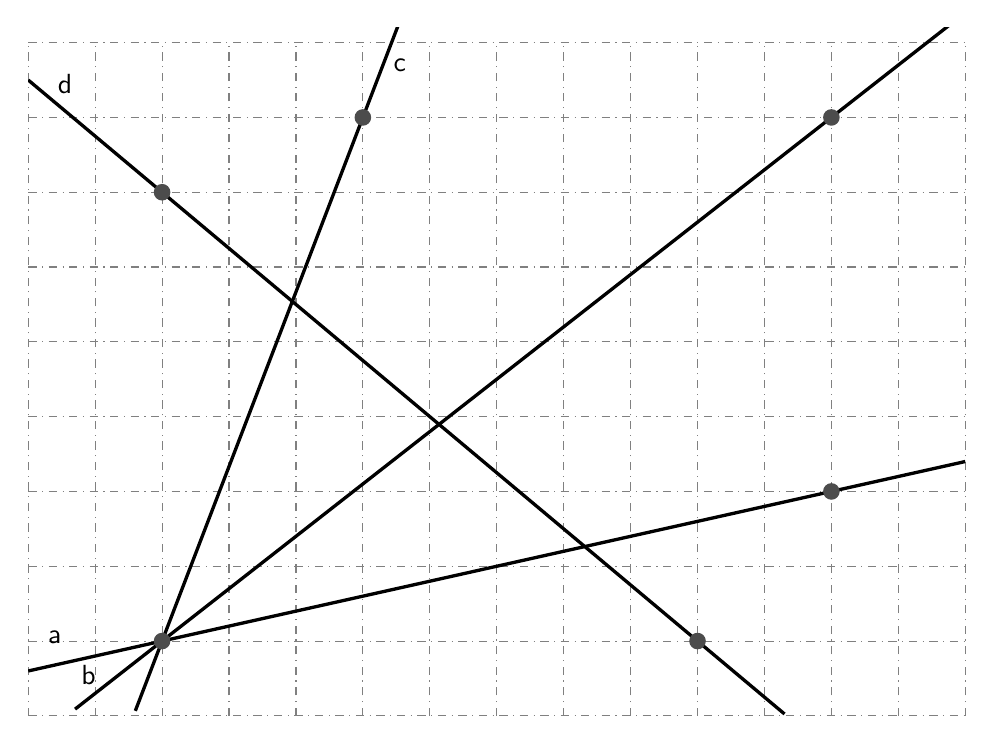
\begin{tikzpicture}[x=0.85cm, y=0.95cm]
            \draw[gray, dash dot, step=1] (-2,-1) grid (12,8);
            \begin{scope}
                \clip (-2,-1) rectangle (12,8.2);
                \draw[very thick] (-2,-0.4) -- (12,2.4);           % a
                \draw[very thick] (-1.3,-0.91) -- (12,8.4);        % b
                \draw[very thick] (-0.4,-0.933) -- (3.6,8.4);      % c
                \draw[very thick] (-2,7.5) -- (9.3,-0.975);        % d
            \end{scope}
            \foreach \p in {(0,0),(10,2),(10,7),(3,7),(0,6),(8,0)}
            \fill[black!70] \p circle (3pt);
            \node[font=\sffamily] at (-1.6,0.05) {a};
            \node[font=\sffamily] at (-1.1,-0.45) {b};
            \node[font=\sffamily] at (3.55,7.7) {c};
            \node[font=\sffamily] at (-1.45,7.45) {d};
        \end{tikzpicture}
    \end{center} 
    \begin{center} 
        \fbox{\parbox{0.95\linewidth}{\centering\Large Erfinden Sie eine Masszahl für \enquote{Steilheit}!}}
    \end{center}
    Können Sie Alice bei diesem Unterfangen helfen? Genauer: Können Sie die Steilheit einer Geraden durch eine einzige Zahl ausdrücken, die Alice dann am Telefon nennen kann? Die Masszahl für Steilheit soll folgenden Regeln genügen:
    \begin{enumerate}
        \item Die Zahl soll für jede mögliche Gerade nach derselben Regel zustande kommen.
        \item Je grösser die Zahl ist, desto steiler ist die Gerade. (Die Grösse der Zahl gibt Bob also eine präzise Vorstellung davon, wie steil die Gerade ist.)
        \item Positive Zahlen stehen für Geraden, die streng monoton wachsen (wie a, b, c), und negative Zahlen stehen für Geraden, die streng monoton fallen (wie d).
        \item Es muss für Alice möglich sein, die Masszahlen für die Geraden a\,--\,d allein aus der abgebildeten Graphik ohne weitere Hilfsmittel präzise zu bestimmen.
    \end{enumerate}
\end{mdframed}
\medskip
Meine Überlegungen, Lösungen:
\kariert{8}
\newpage

\subsection{Was ist eine lineare Funktion?}
In den ersten drei Kapiteln haben Sie gelernt, was Funktionen sind, wie man sie graphisch darstellen kann und welche Eigenschaften des Graphen häufig von Bedeutung sind. Im Folgenden werden Funktionen untersucht, die in der Praxis häufig zur Anwendung kommen. Dabei wird eine ähnliche Strategie wie bei den Gleichungen verfolgt: Funktionen werden nicht einzeln untersucht, sondern gewissen Typen zugeordnet, deren gemeinsame Eigenschaften festgehalten werden. Begonnen wird mit dem einfachsten Funktionstyp: den linearen Funktionen.
\begin{deff}[Lineare Funktion]{def:lineare-funktion}
    Eine Funktion mit einer Funktionsgleichung der Form
    \[f(x) = ax + b\]
    heisst \textbf{lineare Funktion} oder (Polynom-)\textbf{Funktion 1.~Grades}.
\end{deff}

\begin{example}
    Die Funktion $f(x) = 3x + 1$ ist eine lineare Funktion ($a = 3$, $b = 1$).
\end{example}

\begin{example}
    Die Funktion $g(x) = -5 + \dfrac{x}{3}$ ist eine lineare Funktion, denn sie ist von der Form
    \[g(x) = \frac{1}{3} \cdot x + (-5) \qquad \left(a = \tfrac{1}{3},\ b = -5\right).\]
\end{example}

\begin{example}
    Die Funktion $h(x) = x$ ist eine lineare Funktion ($a = 1$, $b = 0$).
\end{example}

\begin{example}
    Bei einer Funktion wie $k(x) = 3$ ist sich die Gemeinschaft der Mathematiker*innen nicht einig, ob sie zu den linearen Funktionen zählen soll. Die einen sagen ja ($a = 0$, $b = 3$), die anderen sagen, dass $a = 0$ nicht zulässig ist.

    Der Einfachheit halber werden wir sie als lineare Funktion betrachten.
\end{example}

\begin{example}
    Die Funktionen $y = x^{2}$, $y = \dfrac{1}{x}$, $y = \sqrt{x}$, $y = 10^{x}$ sind allesamt \textbf{keine} linearen Funktionen.
\end{example}

\textbf{Bemerkung:} Die Parameter $a$ und $b$ werden häufig auch mit $m$ und $q$ bezeichnet.
\bigskip

\begin{minipage}{0.4\textwidth}
    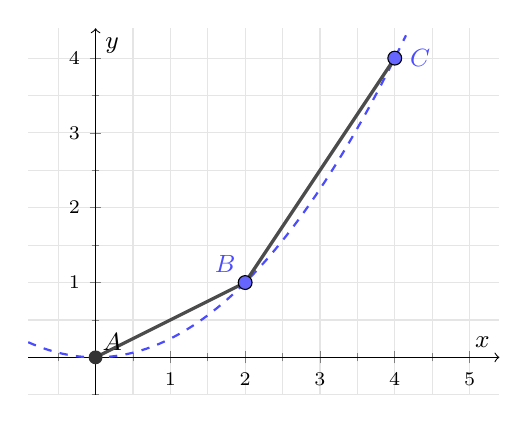
\begin{tikzpicture}
        \begin{axis}[
                linfkt,
                xmin=-0.9, xmax=5.4,
                ymin=-0.5, ymax=4.4,
                minor tick num=1,
                x=0.95cm, y=0.95cm,
            ]
            \addplot[domain=-0.9:4.15, samples=100, smooth, thick, dashed, blue!70] {x^2/4};
            \draw[very thick, black!70] (0,0) -- (2,1) -- (4,4);
            \fill[black!80] (0,0) circle (2.5pt) node[above right=-1pt, black] {\small $A$};
            \fill[blue!60, draw=black] (2,1) circle (2.5pt) node[above left, blue!70] {\small $B$};
            \fill[blue!60, draw=black] (4,4) circle (2.5pt) node[right=2pt, blue!70] {\small $C$};
        \end{axis}
    \end{tikzpicture}
\end{minipage}\hfill
\begin{minipage}{0.56\textwidth}
    Als nächstes soll argumentiert werden, dass die Graphen von linearen Funktionen stets Geraden sind. Zu diesem Zweck wird untersucht, wie steil die Verbindungsstrecken zwischen zwei Graphenpunkten sind. Wenn diese überall gleich steil verlaufen, handelt es sich beim Graphen um eine Gerade.

    \medskip
    Diese Idee versteht man vielleicht besser, wenn man ein Beispiel (links) eines Graphen betrachtet, der keine Gerade ist. Weil die Strecke zwischen den Graphenpunkten $A$ und $B$ weniger steil verläuft als jene zwischen den Graphenpunkten $B$ und $C$, ist der Graph keine Gerade.
\end{minipage}
\medskip

Damit die «Steilheit» zweier Strecken verglichen werden kann, wird eine Masszahl dafür benötigt.

\subsection{Steigung einer Geraden}
\begin{minipage}{0.85\textwidth}
    Hat eine Strasse eine Steigung von 12\,\% bzw. 0.12, bedeutet das, dass die Strasse auf 100 Meter in horizontaler Richtung 12 Meter in vertikaler Richtung ansteigt.
\end{minipage}\hfill
\begin{minipage}{0.12\textwidth}
    \centering
    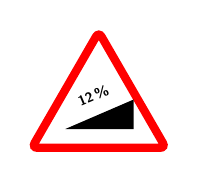
\begin{tikzpicture}[scale=0.85]
        \draw[red, line width=3pt, rounded corners=2pt, fill=white] (0,0) -- (2,0) -- (1,1.732) -- cycle;
        \fill (0.5,0.28) -- (1.52,0.28) -- (1.52,0.72) -- cycle;
        \node[font=\sffamily\bfseries\tiny, rotate=23] at (0.92,0.78) {12\,\%};
    \end{tikzpicture}
\end{minipage}
\medskip

Auf 50 Meter in horizontaler Richtung steigt die Strasse entsprechend um $0.12 \cdot 50 = 6$ Meter an. Auf 42 Meter in horizontaler Richtung beträgt der Anstieg $0.12 \cdot 42 = 5.04$ Meter.

Die Steigung $12\,\% = 0.12$ ist also das Verhältnis des Anstiegs zur Strecke in horizontaler Richtung.

Genauso wird auch die Steigung einer Geraden im Koordinatensystem definiert.
\begin{deff}[Steigung]{def:steigung}
    Sei $g$ eine Gerade im Koordinatensystem durch die Punkte $A = (x_{A},y_{A})$ und $B = (x_{B},y_{B})$. Die \textbf{Steigung} der Geraden $g$ ist definiert als das Verhältnis
    \[\frac{\Delta y}{\Delta x} = \frac{y_{B} - y_{A}}{x_{B} - x_{A}}\]
    \begin{center}
        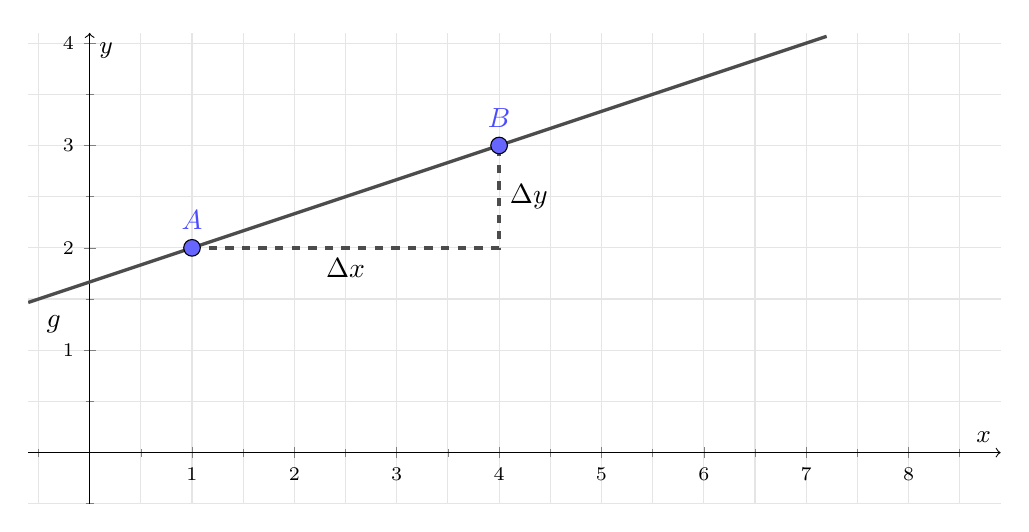
\begin{tikzpicture}
            \begin{axis}[
                    linfkt,
                    xmin=-0.6, xmax=8.9,
                    ymin=-0.5, ymax=4.1,
                    minor tick num=1,
                    x=1.3cm, y=1.3cm,
                ]
                \addplot[domain=-0.6:7.2, very thick, black!70] {x/3+5/3};
                \draw[very thick, dashed, black!70] (1,2) -- node[below, black] {$\Delta x$} (4,2) -- node[right, black] {$\Delta y$} (4,3);
                \fill[blue!60, draw=black] (1,2) circle (3pt) node[above=3pt, blue!70] {$A$};
                \fill[blue!60, draw=black] (4,3) circle (3pt) node[above=3pt, blue!70] {$B$};
                \node at (-0.35,1.25) {$g$};
            \end{axis}
        \end{tikzpicture}
    \end{center}
\end{deff}

\newpage
\textbf{Bemerkungen:}
\begin{itemize}
    \item Das Symbol $\Delta$ ist der griechische Grossbuchstabe «Delta» und steht für «Differenz». Die Steigung ist das Verhältnis der Differenz der $y$-Koordinaten zur Differenz der $x$-Koordinaten.
    \item Die Gerade im Bild oben hat die Steigung $\dfrac{\Delta y}{\Delta x} = \dfrac{3 - 2}{4 - 1} = \dfrac{1}{3}$.
    \item \begin{minipage}[t]{0.5\linewidth}
              Es spielt keine Rolle, welche zwei Punkte der Geraden zur Ermittlung der Steigung verwendet werden. Die Steigung der Geraden im Bild oben hätte man auch wie folgt bestimmen können:
              \[\frac{\Delta y}{\Delta x} = \frac{4 - 2}{7 - 1} = \frac{2}{6} = \frac{1}{3}\]
              Weil die beiden verwendeten Dreiecke -- die sogenannten \textit{Steigungsdreiecke} -- ähnlich sind, ist das Verhältnis der beiden Katheten in beiden gleich.
          \end{minipage}\hfill
          \begin{minipage}[t]{0.46\linewidth}
              \vspace{0pt}
              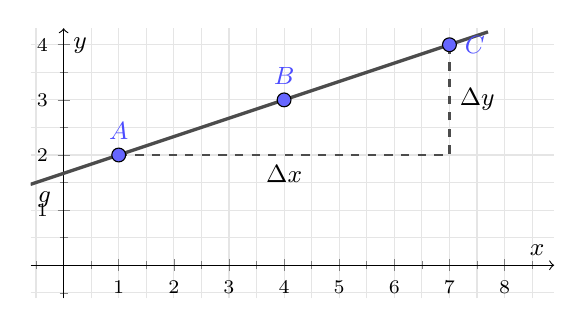
\begin{tikzpicture}
                  \begin{axis}[
                          linfkt,
                          xmin=-0.6, xmax=8.9,
                          ymin=-0.6, ymax=4.3,
                          minor tick num=1,
                          x=0.7cm, y=0.7cm,
                      ]
                      \addplot[domain=-0.6:7.7, very thick, black!70] {x/3+5/3};
                      \draw[thick, dashed, black!70] (1,2) -- node[below, black] {\small $\Delta x$} (7,2) -- node[right, black] {\small $\Delta y$} (7,4);
                      \fill[blue!60, draw=black] (1,2) circle (2.5pt) node[above=2pt, blue!70] {\small $A$};
                      \fill[blue!60, draw=black] (4,3) circle (2.5pt) node[above=2pt, blue!70] {\small $B$};
                      \fill[blue!60, draw=black] (7,4) circle (2.5pt) node[right=2pt, blue!70] {\small $C$};
                      \node at (-0.35,1.2) {\small $g$};
                  \end{axis}
              \end{tikzpicture}
          \end{minipage}
          \bigskip

    \item \begin{minipage}[t]{0.5\linewidth}
              Eine Gerade ist genau dann streng monoton wachsend (bzw. fallend), wenn ihre Steigung positiv (bzw. negativ) ist.

              \medskip
              \textit{Beispiel:} Die Gerade im Bild hat die Steigung
              \begin{align*}
                  \frac{\Delta y}{\Delta x} & = \frac{y_{B} - y_{A}}{x_{B} - x_{A}} = \frac{-2 - 2}{7 - 1} \\[1mm]
                                            & = \frac{-4}{6} = -\frac{2}{3}
              \end{align*}
          \end{minipage}\hfill
          \begin{minipage}[t]{0.46\linewidth}
              \vspace{0pt}
              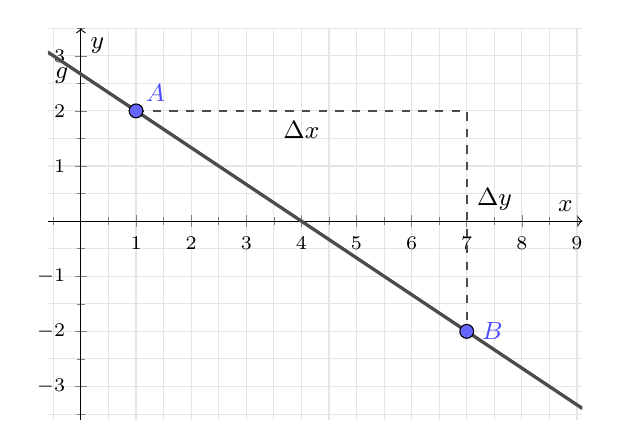
\begin{tikzpicture}
                  \begin{axis}[
                          linfkt,
                          xmin=-0.6, xmax=9.1,
                          ymin=-3.6, ymax=3.5,
                          minor tick num=1,
                          x=0.7cm, y=0.7cm,
                      ]
                      \addplot[domain=-0.6:9.1, very thick, black!70] {-2/3*x+8/3};
                      \draw[thick, dashed, black!70] (1,2) -- node[below, black] {\small $\Delta x$} (7,2) -- node[right, black, pos=0.4] {\small $\Delta y$} (7,-2);
                      \fill[blue!60, draw=black] (1,2) circle (2.5pt) node[above right, blue!70] {\small $A$};
                      \fill[blue!60, draw=black] (7,-2) circle (2.5pt) node[right=2pt, blue!70] {\small $B$};
                      \node at (-0.35,2.65) {\small $g$};
                  \end{axis}
              \end{tikzpicture}
          \end{minipage}
          \bigskip

    \item \begin{minipage}[t]{0.5\linewidth}
              Eine Gerade mit der Steigung $1 = 100\,\%$ ist um $45^\circ$ gegenüber der Horizontalen geneigt.
              \begin{align*}
                  \frac{\Delta y}{\Delta x} & = \frac{y_{B} - y_{A}}{x_{B} - x_{A}} = \frac{-1.5 - (-3)}{2.5 - 1} \\[1mm]
                                            & = \frac{1.5}{1.5} = 1 = 100\,\%
              \end{align*}
          \end{minipage}\hfill
          \begin{minipage}[t]{0.46\linewidth}
              \vspace{0pt}
              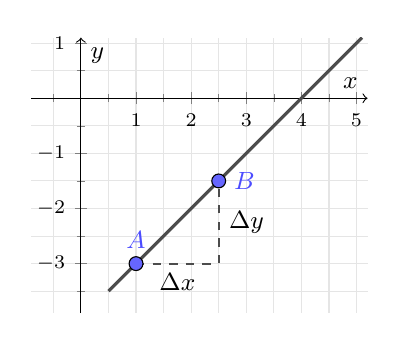
\begin{tikzpicture}
                  \begin{axis}[
                          linfkt,
                          xmin=-0.9, xmax=5.2,
                          ymin=-3.9, ymax=1.1,
                          minor tick num=1,
                          x=0.7cm, y=0.7cm,
                      ]
                      \addplot[domain=0.5:5.1, very thick, black!70] {x-4};
                      \draw[thick, dashed, black!70] (1,-3) -- node[below, black] {\small $\Delta x$} (2.5,-3) -- node[right, black] {\small $\Delta y$} (2.5,-1.5);
                      \fill[blue!60, draw=black] (1,-3) circle (2.5pt) node[above=2pt, blue!70] {\small $A$};
                      \fill[blue!60, draw=black] (2.5,-1.5) circle (2.5pt) node[right=2pt, blue!70] {\small $B$};
                  \end{axis}
              \end{tikzpicture}
          \end{minipage}
          \bigskip

    \item Für vertikale Geraden gilt $\Delta x = 0$. Aus diesem Grund hat eine vertikale Gerade keine Steigung.
\end{itemize}

\begin{fazit}[Merkspruch]{}
    Steigung = «Obsi pro Vorwärts»
\end{fazit}
\newpage

\subsection{Der Graph einer linearen Funktion}
\subsubsection{Einführungsaufgaben}
\begin{enumerate}
    \item Liegen die Punkte $A = (1,2)$, $B = (8,4)$ und $C = (18,7)$ auf einer Geraden? Tipp: Betrachten Sie die Steigung.
    \item Gegeben ist die Funktion $f(x) = 2x + 6$.
          \begin{enumerate}
              \item Bestimmen Sie die Koordinaten von drei Punkten auf dem Graphen von $f$. Zeigen Sie, dass sie auf einer Geraden liegen.
              \item Wieso reicht die Aufgabe a) nicht als Beweis dafür, dass der Graph von $f$ eine Gerade ist?
              \item Challenge: Betrachten Sie nun zwei allgemeine Punkte $A = (x_{A},y_{A})$ und $B = (x_{B},y_{B})$ auf dem Graphen von $f$.
                    \begin{enumerate}[label=\roman*)]
                        \item Erklären Sie, wieso $y_{A} = 2x_{A} + 6$ sein muss.
                        \item Berechnen Sie die Steigung und formen Sie den Term so lange um, bis Sie eine Zahl erhalten.
                    \end{enumerate}
          \end{enumerate}
\end{enumerate}

\begin{theo}[Graph einer linearen Funktion]{satz:graph-lineare-funktion}
    Der Graph einer linearen Funktion der Form $f(x) = ax + b$ ist eine Gerade mit dem $y$-Achsen\-abschnitt $b$ und der Steigung $a$.
    \begin{center}
        \begin{tikzpicture}[>=stealth, scale=0.9]
            \draw[->] (-4.4,0) -- (8,0);
            \draw[->] (0,-1.2) -- (0,4.1);
            \draw[very thick, black!70] (-4.4,-0.12) -- (8,3.6);
            \draw[very thick, black!70] (0,1.2) -- node[below, black] {$\Delta x$} (3.8,1.2) -- node[right, black] {$\Delta y$} (3.8,2.34);
            \fill (0,1.2) circle (1.5pt) node[above left] {$b$};
            \node at (5.7,1.0) {$\dfrac{\Delta y}{\Delta x} = a$};
            \node at (-2.3,-0.8) {$f(x) = ax + b$};
        \end{tikzpicture}
    \end{center}
\end{theo}

\begin{prf}
    Zuerst wird bewiesen, dass der $y$-Achsen\-abschnitt $b$ ist. Zur Erinnerung: Der $y$-Achsen\-abschnitt ist der Funktionswert an der Stelle $0$. In diesem Fall also:
    \[f(0) = a \cdot 0 + b = b\]
    Nun wird gezeigt, dass der Graph von $f$ eine Gerade ist: Seien $A = (x_{A},y_{A})$ und $B = (x_{B},y_{B})$ zwei \textit{beliebige} Punkte auf dem Graphen von $f$. Das heisst: $y_{A} = f(x_{A})$ und $y_{B} = f(x_{B})$. Die Steigung der Verbindungsstrecke zwischen $A$ und $B$ beträgt dann:
    \begin{align*}
        \frac{\Delta y}{\Delta x} & = \frac{y_{B} - y_{A}}{x_{B} - x_{A}} = \frac{f(x_{B}) - f(x_{A})}{x_{B} - x_{A}}                                                                             \\[1mm]
                                  & = \frac{(a \cdot x_{B} + b) - (a \cdot x_{A} + b)}{x_{B} - x_{A}} = \frac{a \cdot x_{B} - a \cdot x_{A}}{x_{B} - x_{A}} = \frac{a \cdot (x_{B} - x_{A})}{x_{B} - x_{A}} = a
    \end{align*}
    Die Steigung zwischen zwei Graphenpunkten ist demnach immer dieselbe, nämlich $a$. Damit muss der Graph eine Gerade mit der Steigung $a$ sein. \hfill $\blacksquare$
\end{prf}
\newpage

\subsection{Übungen}
\begin{enumerate}
    \item Zeichnen Sie die Gerade mit der angegebenen Funktionsgleichung ohne Wertetabelle, nur mit Hilfe des $y$-Achsenabschnitts $q$ und der Steigung $m$ in ein Koordinatensystem ein.
          \begin{multicols}{4}
              \begin{enumerate}
                  \item $y = 2x + 3$
                  \item $y = -3x - 1$
                  \item $y = \frac{3}{5}x + \frac{5}{2}$
                  \item $y = -\frac{5}{3}x - \frac{2}{5}$
              \end{enumerate}
          \end{multicols}
    \item Geben Sie für jede Gerade die Funktionsgleichung an.
          \begin{multicols}{2}
              \begin{enumerate}
                  \item 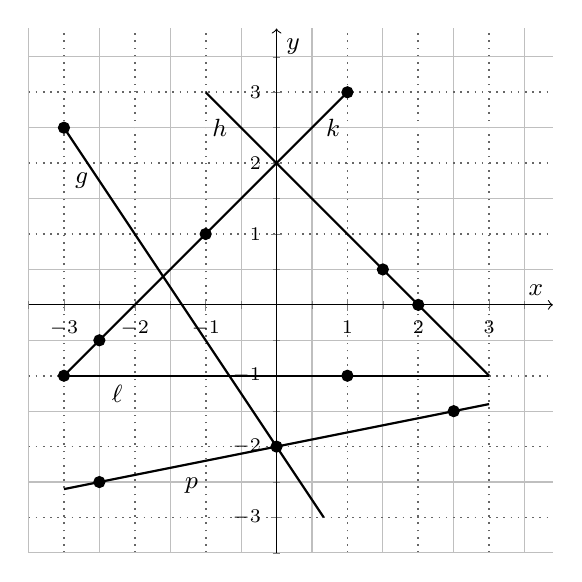
\begin{tikzpicture}[baseline=(current bounding box.north)]
                            \begin{axis}[
                                    linfktpunkt,
                                    xmin=-3.5, xmax=3.9,
                                    ymin=-3.5, ymax=3.9,
                                    minor tick num=1,
                                    x=0.9cm, y=0.9cm,
                                ]
                                \addplot[domain=-3:0.667, thick] {-1.5*x-2};
                                \addplot[domain=-1:3, thick] {-x+2};
                                \addplot[domain=-3:1, thick] {x+2};
                                \addplot[domain=-3:3, thick] {-1};
                                \addplot[domain=-3:3, thick] {0.2*x-2};
                                \addplot[only marks, mark=*, mark size=2pt] coordinates {(-3,2.5) (0,-2) (1.5,0.5) (2,0) (-2.5,-0.5) (-1,1) (1,3) (-3,-1) (1,-1) (-2.5,-2.5) (2.5,-1.5)};
                                \node at (-2.75,1.75) {\small $g$};
                                \node at (-0.8,2.5) {\small $h$};
                                \node at (0.8,2.5) {\small $k$};
                                \node at (-2.25,-1.25) {\small $\ell$};
                                \node at (-1.2,-2.55) {\small $p$};
                            \end{axis}
                        \end{tikzpicture}
                  \item 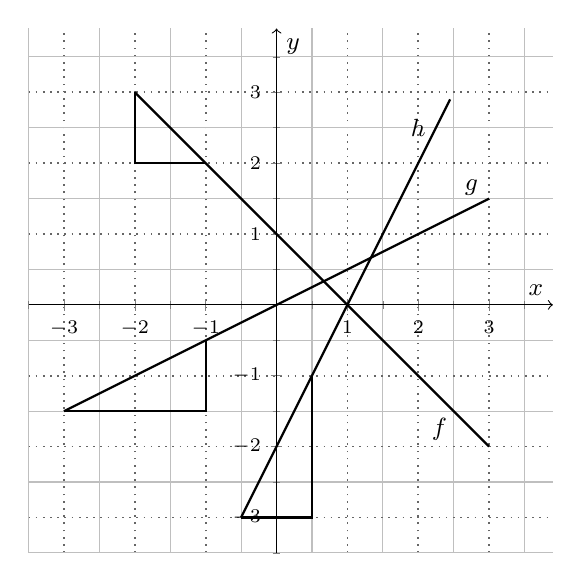
\begin{tikzpicture}[baseline=(current bounding box.north)]
                            \begin{axis}[
                                    linfktpunkt,
                                    xmin=-3.5, xmax=3.9,
                                    ymin=-3.5, ymax=3.9,
                                    minor tick num=1,
                                    x=0.9cm, y=0.9cm,
                                ]
                                \addplot[domain=-2:3, thick] {-x+1};
                                \addplot[domain=-3:3, thick] {0.5*x};
                                \addplot[domain=-0.5:2.45, thick] {2*x-2};
                                \draw[thick] (-2,3) -- (-2,2) -- (-1,2);
                                \draw[thick] (-3,-1.5) -- (-1,-1.5) -- (-1,-0.5);
                                \draw[thick] (-0.5,-3) -- (0.5,-3) -- (0.5,-1);
                                \node at (2.3,-1.75) {\small $f$};
                                \node at (2.75,1.65) {\small $g$};
                                \node at (2,2.5) {\small $h$};
                            \end{axis}
                        \end{tikzpicture}
              \end{enumerate}
          \end{multicols}
\end{enumerate}

\subsubsection{Lösungen}
\begin{enumerate}
    \item \begin{multicols}{4}
              \begin{enumerate}
                  \item 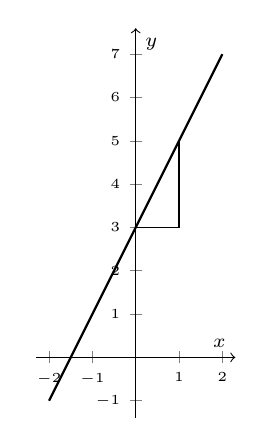
\begin{tikzpicture}[baseline=(current bounding box.north)]
                            \begin{axis}[
                                    axis lines=middle, axis line style={->},
                                    xlabel={$x$}, ylabel={$y$},
                                    x=0.55cm, y=0.55cm,
                                    xmin=-2.3, xmax=2.3, ymin=-1.4, ymax=7.6,
                                    xtick distance=1, ytick distance=1,
                                    tick label style={font=\tiny}, label style={font=\scriptsize},
                                    enlargelimits=false,
                                ]
                                \addplot[domain=-2:2, thick] {2*x+3};
                                \draw (0,3) -- (1,3) -- (1,5);
                            \end{axis}
                        \end{tikzpicture}
                  \item 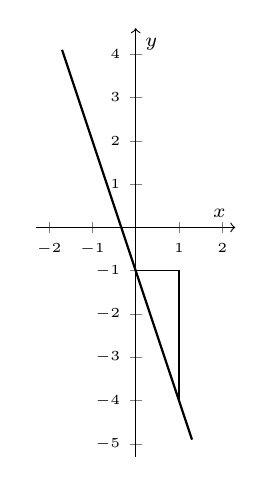
\begin{tikzpicture}[baseline=(current bounding box.north)]
                            \begin{axis}[
                                    axis lines=middle, axis line style={->},
                                    xlabel={$x$}, ylabel={$y$},
                                    x=0.55cm, y=0.55cm,
                                    xmin=-2.3, xmax=2.3, ymin=-5.3, ymax=4.6,
                                    xtick distance=1, ytick distance=1,
                                    tick label style={font=\tiny}, label style={font=\scriptsize},
                                    enlargelimits=false,
                                ]
                                \addplot[domain=-1.7:1.3, thick] {-3*x-1};
                                \draw (0,-1) -- (1,-1) -- (1,-4);
                            \end{axis}
                        \end{tikzpicture}
                  \item 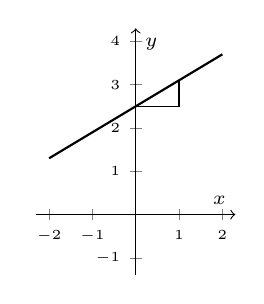
\begin{tikzpicture}[baseline=(current bounding box.north)]
                            \begin{axis}[
                                    axis lines=middle, axis line style={->},
                                    xlabel={$x$}, ylabel={$y$},
                                    x=0.55cm, y=0.55cm,
                                    xmin=-2.3, xmax=2.3, ymin=-1.4, ymax=4.3,
                                    xtick distance=1, ytick distance=1,
                                    tick label style={font=\tiny}, label style={font=\scriptsize},
                                    enlargelimits=false,
                                ]
                                \addplot[domain=-2:2, thick] {0.6*x+2.5};
                                \draw (0,2.5) -- (1,2.5) -- (1,3.1);
                            \end{axis}
                        \end{tikzpicture}
                  \item 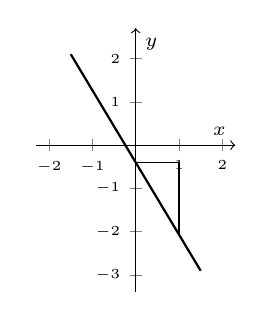
\begin{tikzpicture}[baseline=(current bounding box.north)]
                            \begin{axis}[
                                    axis lines=middle, axis line style={->},
                                    xlabel={$x$}, ylabel={$y$},
                                    x=0.55cm, y=0.55cm,
                                    xmin=-2.3, xmax=2.3, ymin=-3.4, ymax=2.7,
                                    xtick distance=1, ytick distance=1,
                                    tick label style={font=\tiny}, label style={font=\scriptsize},
                                    enlargelimits=false,
                                ]
                                \addplot[domain=-1.5:1.5, thick] {-5/3*x-0.4};
                                \draw (0,-0.4) -- (1,-0.4) -- (1,-2.0667);
                            \end{axis}
                        \end{tikzpicture}
              \end{enumerate}
          \end{multicols}
    \item \begin{enumerate}
              \item $g(x) = -\frac{3}{2}x - 2$, \quad $h(x) = -x + 2$, \quad $k(x) = x + 2$, \quad $\ell(x) = -1$, \quad $p(x) = \frac{1}{5}x - 2$
              \item $f(x) = -x + 1$, \quad $g(x) = \frac{1}{2}x$, \quad $h(x) = 2x - 2$
          \end{enumerate}
\end{enumerate}
\newpage

\subsection{Funktionsgleichung $\leftrightarrow$ Graph}
\begin{example}
    \textbf{Gegeben} ist die Funktionsgleichung $f(x) = -\dfrac{2}{3}x + 1$.

    \textbf{Gesucht} ist der Graph der Funktion.
    \kariert{15}
\end{example}

\begin{example}
    \textbf{Gegeben} sind zwei Punkte $P = (0,1)$ und $Q = (2,4)$ auf dem Graphen der linearen Funktion $g$.

    \textbf{Gesucht} ist die Funktionsgleichung.
    \kariert{22}
\end{example}
\newpage

\begin{example}
    \textbf{Notenskala:} Bei einer Prüfung erhält man für 0 Punkte die Note 1, für 17 Punkte die Note 6. Dazwischen ist die Notenskala linear.

    Wie lautet die Gleichung der Funktion
    \[N: [0,17] \to [1,6],\]
    die jeder Punktzahl $p$ die entsprechende Note $N(p)$ zuordnet?
    \kariert{40}
\end{example}
\newpage

\begin{example}
    Für welche lineare Funktion $f$ gilt $f(1) = 2$ und $f(6) = 5$?
    \kariert{38}
\end{example}
\newpage

\subsection{Übungen}
\begin{enumerate}
    \item Die Punkte $A$ und $B$ liegen auf einer Geraden. Geben Sie deren Funktionsgleichung an.
          \begin{multicols}{3}
              \begin{enumerate}
                  \item $A = (-2,5)$, $B = (3,20)$
                  \item $A = (0,0)$, $B = (1,-2)$
                  \item $A = (-7,3)$, $B = (11,3)$
              \end{enumerate}
          \end{multicols}
    \item Von der Funktion $f(x) = y = \frac{2}{3}x + q$ ist $f(-6) = 0$ bekannt. Berechnen Sie $q$ und $f(10)$.
    \item Von der Funktion $f(x) = y = mx + 4$ ist $f(5) = 9$ bekannt. Berechnen Sie $m$ und $f(-5)$.
    \item Eine lineare Funktion hat die Gleichung $f(x) = \frac{1}{3}x - 2$. Bestimmen Sie $f(0)$, $f(-4)$ und $f(27)$. Für welche Stelle $x$ gilt $f(x) = 3$ bzw. $f(x) = -5$?
    \item Gegeben sind die Funktionen $f_{1}: y = -\frac{1}{2}x$, $f_{2}: y = -2x + 2$ und $f_{3}: y = \frac{5}{2}x - \frac{2}{3}$.
          \begin{enumerate}
              \item Welche Funktion hat als Graph eine Gerade durch $(0,0)$?
              \item Welche Funktion hat als Graph eine Gerade mit einer Steigung grösser als $2$?
              \item Welche Funktion hat als Graph eine Gerade parallel zur $x$-Achse?
              \item Schneiden die Graphen der Funktionen $f_{1}$ und $f_{2}$ einander?
          \end{enumerate}
    \item Gegeben sind die Geraden $g: y = 3x$ und $h: y = -\frac{1}{2}x - 1$.
          \begin{enumerate}
              \item Die Graphen von $g$ und $h$ werden an der $y$-Achse gespiegelt. Geben Sie die Funktionsgleichungen der Bildgeraden an.
              \item Die Graphen von $g$ und $h$ werden an der $x$-Achse gespiegelt. Geben Sie die Funktionsgleichungen der Bildgeraden an.
              \item Die Graphen von $g$ und $h$ werden am Koordinatenursprung gespiegelt. Geben Sie die Funktionsgleichungen der Bildgeraden an.
          \end{enumerate}
\end{enumerate}

\subsubsection{Lösungen}
\begin{enumerate}
    \item \begin{multicols}{3}
              \begin{enumerate}
                  \item $f(x) = 3x + 11$
                  \item $f(x) = -2x$
                  \item $f(x) = 3$
              \end{enumerate}
          \end{multicols}
    \item Es ist $q = 4$ und $f(10) = \frac{32}{3}$.
    \item Es ist $m = 1$ und $f(-5) = -1$.
    \item Es ist $f(0) = -2$, $f(-4) = -\frac{10}{3}$ und $f(27) = 7$. Zudem gilt $f(15) = 3$ und $f(-9) = -5$.
    \item \begin{multicols}{4}
              \begin{enumerate}
                  \item $f_{1}$
                  \item $f_{3}$
                  \item Keine
                  \item Ja
              \end{enumerate}
          \end{multicols}
    \item \begin{enumerate}
              \item $g': y = -3x$, \quad $h': y = \frac{1}{2}x - 1$
              \item $g': y = -3x$, \quad $h': y = \frac{1}{2}x + 1$
              \item $g': y = 3x$, \quad $h': y = -\frac{1}{2}x + 1$
          \end{enumerate}
\end{enumerate}
\newpage

\subsection{Gegenseitige Lage von zwei Geraden und Schnittpunkte}
Sie kennen Geraden wahrscheinlich schon aus der Geometrie. Folgender Fakt ist Ihnen sicherlich schon begegnet:
\begin{center}
    \textbf{Zwei Geraden schneiden sich genau dann, wenn sie nicht parallel sind.}
\end{center}
Da die Graphen von linearen Funktionen Geraden sind, lässt sich dieser Sachverhalt auch auf diese übertragen. Zuerst untersuchen wir, wann zwei Geraden parallel zueinander sind. Danach sehen wir, wie wir Schnittpunkte der Graphen von linearen Funktionen berechnen.

\subsubsection{Gegenseitige Lage}
\begin{minipage}{0.52\textwidth}
    Zwei Geraden $g: y = a_{1}x + b_{1}$ und $p: y = a_{2}x + b_{2}$ sind genau dann parallel, wenn ihre beiden Steigungen gleich sind:
    \[a_{1} = a_{2}\]
    In der Skizze rechts haben beide abgebildeten Geraden die Steigung $a = -\dfrac{1}{2}$.
\end{minipage}\hfill
\begin{minipage}{0.44\textwidth}
    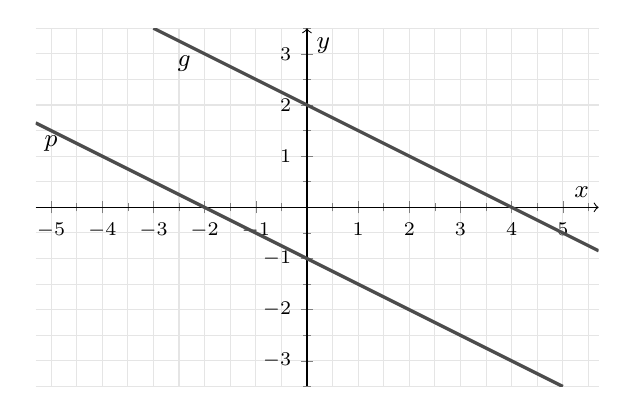
\begin{tikzpicture}
        \begin{axis}[
                linfkt,
                xmin=-5.3, xmax=5.7,
                ymin=-3.5, ymax=3.5,
                minor tick num=1,
                x=0.65cm, y=0.65cm,
            ]
            \addplot[domain=-3:5.7, very thick, black!70] {-0.5*x+2};
            \addplot[domain=-5.3:5, very thick, black!70] {-0.5*x-1};
            \node at (-2.4,2.8) {\small $g$};
            \node at (-5,1.25) {\small $p$};
        \end{axis}
    \end{tikzpicture}
\end{minipage}

\subsubsection{Schnittpunkt}
\begin{minipage}{0.52\textwidth}
    Zwei Geraden seien durch ihre Gleichungen gegeben:
    \[g: y = -\frac{1}{2}x + 2 \quad \text{und} \quad k: y = 2x - \frac{1}{3}\]
    Die Koordinaten $(x_{S},y_{S})$ des Schnittpunktes $S$ lassen sich auf algebraische Weise bestimmen:
\end{minipage}\hfill
\begin{minipage}{0.44\textwidth}
    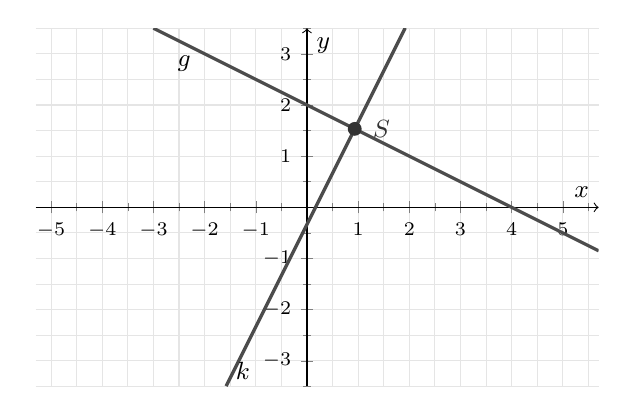
\begin{tikzpicture}
        \begin{axis}[
                linfkt,
                xmin=-5.3, xmax=5.7,
                ymin=-3.5, ymax=3.5,
                minor tick num=1,
                x=0.65cm, y=0.65cm,
            ]
            \addplot[domain=-3:5.7, very thick, black!70] {-0.5*x+2};
            \addplot[domain=-1.58:1.92, very thick, black!70] {2*x-1/3};
            \fill[black!80] (14/15,23/15) circle (2.5pt) node[right=3pt] {\small $S$};
            \node at (-2.4,2.8) {\small $g$};
            \node at (-1.25,-3.2) {\small $k$};
        \end{axis}
    \end{tikzpicture}
\end{minipage}
\medskip

$S$ liegt auf der Geraden $g$. Das ist genau dann der Fall, wenn $y_{S} = -\frac{1}{2}x_{S} + 2$ ist.

$S$ liegt auf der Geraden $k$. Das ist genau dann der Fall, wenn $y_{S} = 2x_{S} - \frac{1}{3}$ ist.
\medskip

Daraus folgt die Gleichung:
\begin{align*}
    -\frac{1}{2}x_{S} + 2 & = 2x_{S} - \frac{1}{3} &  & |\cdot 6             \\
    -3x_{S} + 12          & = 12x_{S} - 2          &  & |+ 3x_{S} + 2        \\
    14                    & = 15x_{S}              &  & |\cdot \tfrac{1}{15} \\
    \frac{14}{15}         & = x_{S}
\end{align*}
Die $y$-Koordinate des Schnittpunktes kann berechnet werden, indem man die $x$-Koordinate in eine der Geradengleichungen einsetzt:
\[y_{S} = -\frac{1}{2} \cdot \frac{14}{15} + 2 = \frac{23}{15} \quad \Rightarrow \quad S = \left( \frac{14}{15},\frac{23}{15} \right)\]
\newpage

\subsection{Übungen}
\begin{enumerate}
    \item Gegeben ist die Gerade $g$ mit der Funktionsgleichung $g: y = -2.5x + 4$. Geben Sie die Gleichung derjenigen Geraden an, die zu $g$ parallel ist und
          \begin{enumerate}
              \item durch den Koordinatenursprung geht.
              \item durch den Punkt $P = (4,1)$ verläuft.
              \item die $x$-Achse eine Einheit weiter rechts schneidet als $g$.
          \end{enumerate}
    \item Gegeben sind die beiden Geraden $g: y = \frac{2}{3}x + \frac{20}{3}$ und $h: y = -\frac{2}{11}x + 2$.
          \begin{enumerate}
              \item Berechnen Sie die Koordinaten des Schnittpunktes $S$ von $g$ und $h$.
              \item Berechnen Sie den Flächeninhalt $F$ des Dreiecks, das $g$ und $h$ zusammen mit der $x$-Achse einschliessen.
          \end{enumerate}
    \item Bestimmen Sie rechnerisch die Koordinaten der drei Schnittpunkte der skizzierten Graphen.
          \begin{multicols}{2}
              \begin{enumerate}
                  \item 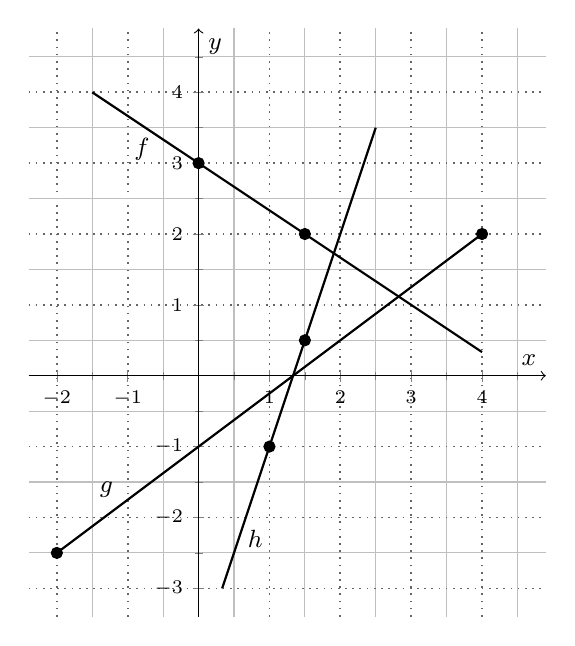
\begin{tikzpicture}[baseline=(current bounding box.north)]
                            \begin{axis}[
                                    linfktpunkt,
                                    xmin=-2.4, xmax=4.9,
                                    ymin=-3.4, ymax=4.9,
                                    minor tick num=1,
                                    x=0.9cm, y=0.9cm,
                                ]
                                \addplot[domain=-1.5:4, thick] {-2/3*x+3};
                                \addplot[domain=-2:4, thick] {0.75*x-1};
                                \addplot[domain=0.333:2.5, thick] {3*x-4};
                                \addplot[only marks, mark=*, mark size=2pt] coordinates {(0,3) (1.5,2) (-2,-2.5) (4,2) (1,-1) (1.5,0.5)};
                                \node at (-0.8,3.2) {\small $f$};
                                \node at (-1.3,-1.6) {\small $g$};
                                \node at (0.8,-2.3) {\small $h$};
                            \end{axis}
                        \end{tikzpicture}
                  \item 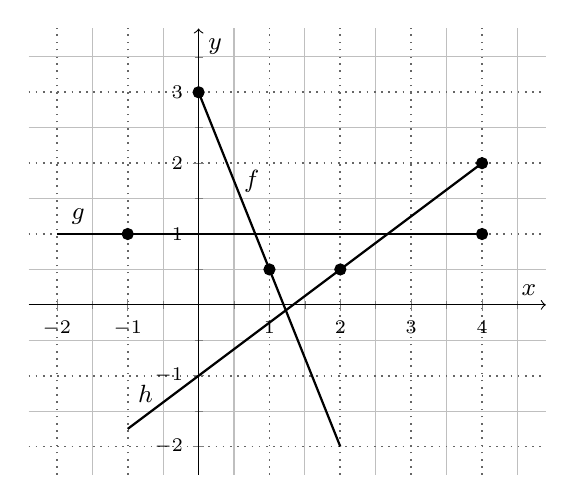
\begin{tikzpicture}[baseline=(current bounding box.north)]
                            \begin{axis}[
                                    linfktpunkt,
                                    xmin=-2.4, xmax=4.9,
                                    ymin=-2.4, ymax=3.9,
                                    minor tick num=1,
                                    x=0.9cm, y=0.9cm,
                                ]
                                \addplot[domain=0:2, thick] {-2.5*x+3};
                                \addplot[domain=-2:4, thick] {1};
                                \addplot[domain=-1:4, thick] {0.75*x-1};
                                \addplot[only marks, mark=*, mark size=2pt] coordinates {(0,3) (1,0.5) (-1,1) (4,1) (2,0.5) (4,2)};
                                \node at (0.75,1.75) {\small $f$};
                                \node at (-1.7,1.25) {\small $g$};
                                \node at (-0.75,-1.25) {\small $h$};
                            \end{axis}
                        \end{tikzpicture}
              \end{enumerate}
          \end{multicols}
\end{enumerate}

\subsubsection{Lösungen}
\begin{enumerate}
    \item \begin{multicols}{3}
              \begin{enumerate}
                  \item $y = -2.5x$
                  \item $y = -2.5x + 11$
                  \item $y = -2.5x + 6.5$
              \end{enumerate}
          \end{multicols}
    \item \begin{multicols}{3}
              \begin{enumerate}
                  \item $S = \left( -\frac{11}{2},3 \right)$
                  \item $F = \frac{63}{2} = 31.5$
              \end{enumerate}
          \end{multicols}
    \item \begin{enumerate}
              \item $S_{fg} = \left( \frac{48}{17},\frac{19}{17} \right)$, \quad $S_{fh} = \left( \frac{21}{11},\frac{19}{11} \right)$, \quad $S_{gh} = \left( \frac{4}{3},0 \right)$
              \item $S_{fg} = \left( \frac{4}{5},1 \right)$, \quad $S_{fh} = \left( \frac{16}{13},-\frac{1}{13} \right)$, \quad $S_{gh} = \left( \frac{8}{3},1 \right)$
          \end{enumerate}
\end{enumerate}
\newpage

\subsection{Lineare Funktionen in Anwendungen}
Ganz am Anfang des Themas Funktionen wurde erwähnt, dass es sich dabei um «mentale Werkzeuge» handelt. Damit ist gemeint, dass man viele Fragestellungen mit einer «Funktionenbrille» betrachten kann und dann Analogien zwischen Problemen entstehen, die auf den ersten Blick nicht viel gemeinsam haben. Eine wesentliche Grundlage des Erfolgs von Newton in der Mechanik beruht darauf, dass er Bewegung als eine Funktion betrachtet hat:

\subsubsection*{Warm-up: Weg-Zeit-Diagramm}
\begin{center}
    \begin{tikzpicture}[>=stealth]
        % Zahlenstrahl mit Figur
        \draw[->] (-0.8,0) -- (5.3,0);
        \foreach \x in {0,1,2,3,4,5}
        \draw (\x,0.1) -- (\x,-0.1) node[below] {\small \x};
        \begin{scope}[shift={(1,0.2)}, thick]
            \draw (0,0.75) circle (0.13);
            \draw (0,0.62) -- (0,0.28);
            \draw (-0.2,0.5) -- (0.2,0.5);
            \draw (-0.17,0) -- (0,0.28) -- (0.17,0);
        \end{scope}
        \draw[->, thick] (1.5,0.65) -- (2.3,0.65);
    \end{tikzpicture}

    \medskip
    Funktion: \quad Zeit $t \mapsto$ Position $s$
    \medskip

    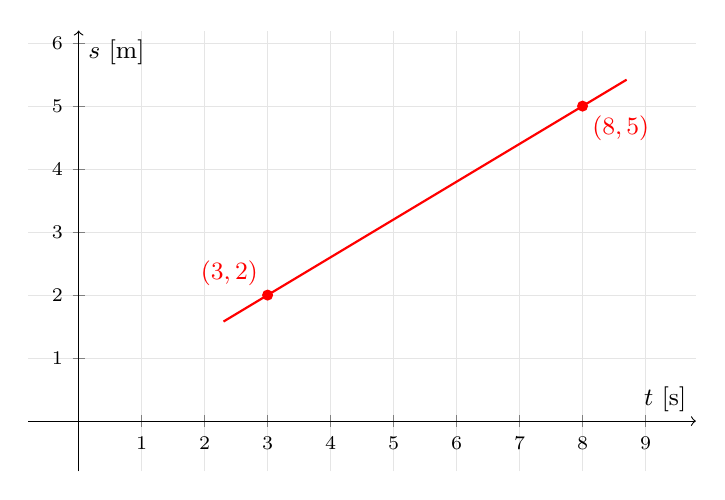
\begin{tikzpicture}
        \begin{axis}[
                axis lines=middle,
                axis line style={->},
                xlabel={$t$ [s]}, ylabel={$s$ [m]},
                xmin=-0.8, xmax=9.8,
                ymin=-0.8, ymax=6.2,
                xtick distance=1, ytick distance=1,
                grid=both,
                grid style={lightgray!40},
                tick label style={font=\scriptsize},
                label style={font=\small},
                enlargelimits=false,
                x=0.8cm, y=0.8cm,
            ]
            \addplot[domain=2.3:8.7, thick, red] {0.6*x+0.2};
            \fill[red] (3,2) circle (2pt) node[above left] {\small $(3,2)$};
            \fill[red] (8,5) circle (2pt) node[below right] {\small $(8,5)$};
        \end{axis}
    \end{tikzpicture}
\end{center}
\begin{enumerate}
    \item Bedeutung der Graphenpunkte $(3,2)$ und $(8,5)$?
    \item Geschwindigkeit?
\end{enumerate}
\newpage

\subsubsection{Übungen}
\begin{enumerate}
    \item Alice fährt mit dem Elektrovelo mit einer konstanten Geschwindigkeit von $v_{A} = \frac{1}{3}\,\frac{\text{km}}{\text{min}}$ in Richtung Flughafen.

          Zum Zeitpunkt $t = 0$ [min] fährt sie am Ortsausgangsschild bei Winterthur-Töss vorbei.

          Bob will Alice mit dem Roller einholen. Er fährt mit konstanter Geschwindigkeit $v_{B} = \frac{4}{3}\,\frac{\text{km}}{\text{min}}$ und passiert das Ortsausgangsschild 30 Minuten nach Alice.
          \begin{enumerate}
              \item Geben Sie die Gleichung der Funktionen $s_{A}(t)$ und $s_{B}(t)$ an, welche jedem Zeitpunkt $t$ [min] die Entfernung [km] von Alice bzw. Bob vom Ortsausgangsschild zuordnen.
              \item Zeichnen Sie die beiden Graphen in das Koordinatensystem.

                    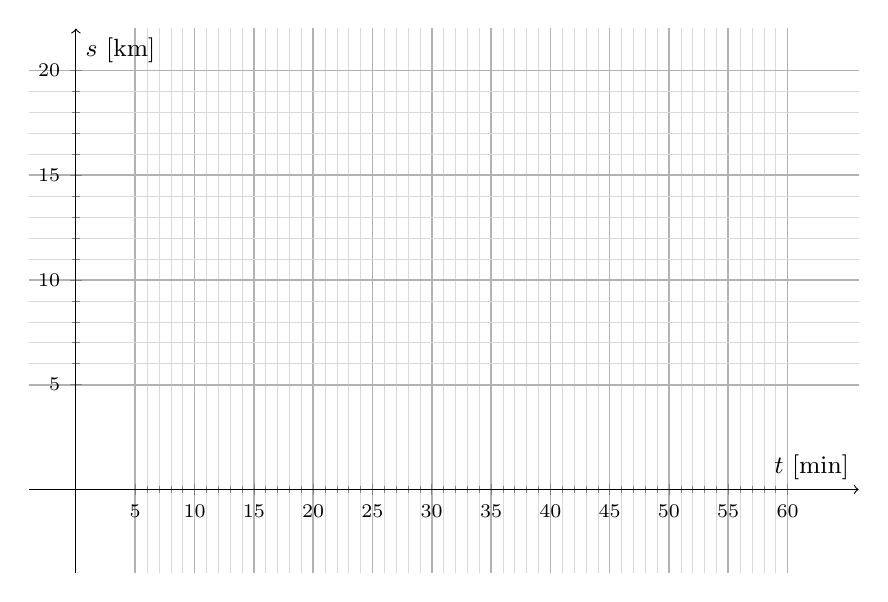
\begin{tikzpicture}
                        \begin{axis}[
                                axis lines=middle,
                                axis line style={->},
                                width=\linewidth, height=8.5cm,
                                xlabel={$t$ [min]}, ylabel={$s$ [km]},
                                xmin=-4, xmax=66,
                                ymin=-4, ymax=22,
                                xtick={5,10,...,60},
                                ytick={5,10,15,20},
                                minor x tick num=4, minor y tick num=4,
                                grid=both,
                                major grid style={line width=0.6pt, draw=gray!60},
                                minor grid style={line width=0.2pt, draw=gray!30},
                                tick label style={font=\scriptsize},
                                label style={font=\small},
                                enlargelimits=false,
                            ]
                        \end{axis}
                    \end{tikzpicture}
              \item Zu welchem Zeitpunkt und in welcher Entfernung von Töss wird Alice von Bob eingeholt? Bzw. schafft es Bob, Alice einzuholen, bevor sie am 13.5 km entfernten Flughafen eintrifft?
          \end{enumerate}
    \item Ein Elektro-Fachgeschäft verkauft verschieden lange Kabel auf identischen Kabelrollen. Eine 20-m-Rolle wiegt 4.2 kg und eine 50-m-Rolle wiegt 9.3 kg. Bestimmen Sie die lineare Funktion $f$, die der Kabellänge $l$ das Gesamtgewicht $G$ der Rolle zuordnet.
    \item In einer Deutschprüfung mit total 34 Punkten ergeben 0 Punkte die Note 1 und 32.5 Punkte die Note 6. Es gibt nur ganze und halbe Punkte und Noten. Die Notenskala ist linear.
          \begin{enumerate}
              \item Geben Sie die Gleichung der Funktion an, die jeder Punktzahl $P$ die Note $N$ zuordnet.
              \item Welche Note erhält Clarissa für 25 Punkte?
              \item Welche Punktzahl benötigt Hans mindestens, um die Note 4 zu erhalten?
          \end{enumerate}
\end{enumerate}
\newpage

\subsubsection{Lösungen}
\begin{enumerate}
    \item \begin{enumerate}
              \item $s_{A}(t) = \frac{1}{3}t$, \quad $s_{B}(t) = \frac{4}{3}t - 40$
              \item 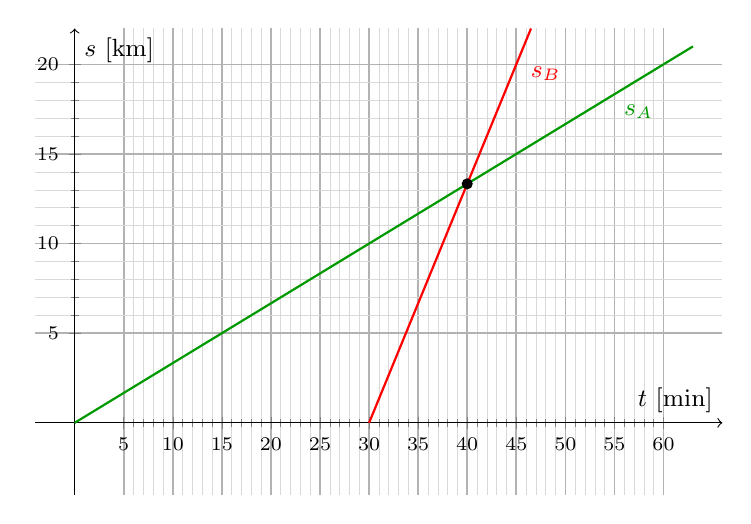
\begin{tikzpicture}[baseline=(current bounding box.north)]
                        \begin{axis}[
                                axis lines=middle,
                                axis line style={->},
                                width=0.85\linewidth, height=7.5cm,
                                xlabel={$t$ [min]}, ylabel={$s$ [km]},
                                xmin=-4, xmax=66,
                                ymin=-4, ymax=22,
                                xtick={5,10,...,60},
                                ytick={5,10,15,20},
                                minor x tick num=4, minor y tick num=4,
                                grid=both,
                                major grid style={line width=0.6pt, draw=gray!60},
                                minor grid style={line width=0.2pt, draw=gray!30},
                                tick label style={font=\scriptsize},
                                label style={font=\small},
                                enlargelimits=false,
                            ]
                            \addplot[domain=0:63, thick, green!60!black] {x/3};
                            \addplot[domain=30:46.5, thick, red] {4/3*x-40};
                            \fill (40,40/3) circle (2pt);
                            \node[green!60!black, below right] at (55,18.3) {\small $s_A$};
                            \node[red, right] at (45.5,19.5) {\small $s_B$};
                        \end{axis}
                    \end{tikzpicture}
              \item Bob holt Alice zum Zeitpunkt $t = 40$ min in der Entfernung $s = \frac{40}{3}$ km $= 13.\overline{3}$ km ein.
          \end{enumerate}
    \item $f: G = 0.17 \cdot l + 0.8$
    \item \begin{enumerate}
              \item $N = \frac{2}{13}P + 1$
              \item $N(25) \approx 4.85$, d.\,h. Note $5$
              \item $P = 17.875$, d.\,h. mindestens $18$ Punkte
          \end{enumerate}
\end{enumerate}
\newpage
